% Standalone notes file. Set as Main Document in Overleaf to compile it alone.
\documentclass[11pt]{article}
\usepackage[margin=1in]{geometry}
\usepackage{graphicx}
\usepackage{subcaption}
\usepackage{amssymb}
\usepackage{enumitem}
\usepackage{array}
\usepackage{booktabs}
\usepackage{hyperref}

\usepackage{xcolor}

\graphicspath{{./}{../}}

% Checkbox list: \item = open box, \item[\done] / \item[\wontfix] = closed.
\newlist{todolist}{itemize}{2}
\setlist[todolist]{label=$\square$, leftmargin=*}
\newcommand{\done}{\rlap{$\square$}{\raisebox{0.5pt}{\hspace{1pt}\tiny$\checkmark$}}}
\newcommand{\wontfix}{\rlap{$\square$}{\hspace{1pt}\tiny$\times$}}

\begin{document}

Motivation: Dynamic shows no benefit on HIGGS - too small. Find bigger datasets.

\begin{figure}[t]
\centering

\includegraphics[width=\linewidth]{figures/intro/dynamic/per_depth_methods_fig1.pdf}
\caption{Per-depth methods.}
\label{fig:motivation}
\end{figure}

\section{Q1. Whats the largest dataset for 24x-metal (384GB RAM)? 48x? m8i.96x (1536GB)?}

\begin{itemize}
    \item HIGGS (11m x 28, 8 GB on disk) peaks at 266GB / 377
    \item EPSILON (400k x 2k , 15.7GB on disk): 257GB training
\end{itemize}

peak dataset on 24x is $\sim$1.4x bigger. $\sim$3x for 48x. 6x for 96x

\subsection{CART}

% Column type: fixed-width, ragged right (no interword stretching).
\newcolumntype{L}[1]{>{\raggedright\arraybackslash}p{#1}}
\begin{table}[htbp]
\centering
\footnotesize
\setlength{\tabcolsep}{4pt}
\renewcommand{\arraystretch}{1.25}
\begin{tabular}{@{}L{1.45cm}L{1.5cm}L{2.05cm}L{1.0cm}L{2.4cm}L{2.5cm}rr@{}}
\toprule
 & \multicolumn{4}{c}{Whole dataset} & \multicolumn{3}{c}{\texttt{m7i.metal-24x} (384\,GB)} \\
\cmidrule(lr){2-5}\cmidrule(lr){6-8}
Dataset & Size & Features & Missing & ML task & Subset that fits & Peak RAM & Train \\
\midrule
\href{https://huggingface.co/datasets/criteo/CriteoClickLogs}{Criteo 1B}
 & $\sim$1B $\times$ 39; 276\,GB raw$^{\ast}$
 & 13 of 39 numeric
 & ---
 & ---
 & Day 1 only: 24.5M $\times$ 39 ($\frac{1}{8}$ of rows)
 & 193\,GB & 747\,s \\
\href{https://www.nyc.gov/site/tlc/about/tlc-trip-record-data.page}{NYC Taxi Trips}
 & 170M $\times$ 20 per year
 & 19 numerical
 & ---
 & \texttt{trip\_duration} (regression)
 & 49.1M $\times$ 18 ($\frac{1}{2}$ fits)
 & 276\,GB & 1070\,s$^{\dagger}$ \\
\href{https://numer.ai/data}{Numerai} v5
 & 5M $\times$ 2{,}376
 & int8, hand-built financial (not embeddings)
 & 0.5--1.29\%
 & \texttt{Target} (regression)
 & full dataset
 & 116\,GB & 561\,s \\
\href{https://transtats.bts.gov/Fields.asp?gnoyr_VQ=FGJ}{Airline on-time}
 & 200M $\times$ 13--70
 & 70 float64, 21 int64, 19 string
 & $\sim$3\%, few cols
 & \texttt{arrival\_delay} (regression)
 & 2018--2023: 37.9M $\times$ 43
 & 342\,GB & 1007\,s \\
\bottomrule
\end{tabular}
\caption{Train Time is Dynamic Vectorized AVX-2 (64-bins)}
\label{tab:cart-datasets}
\end{table}

\begin{figure}[h]
    \centering
    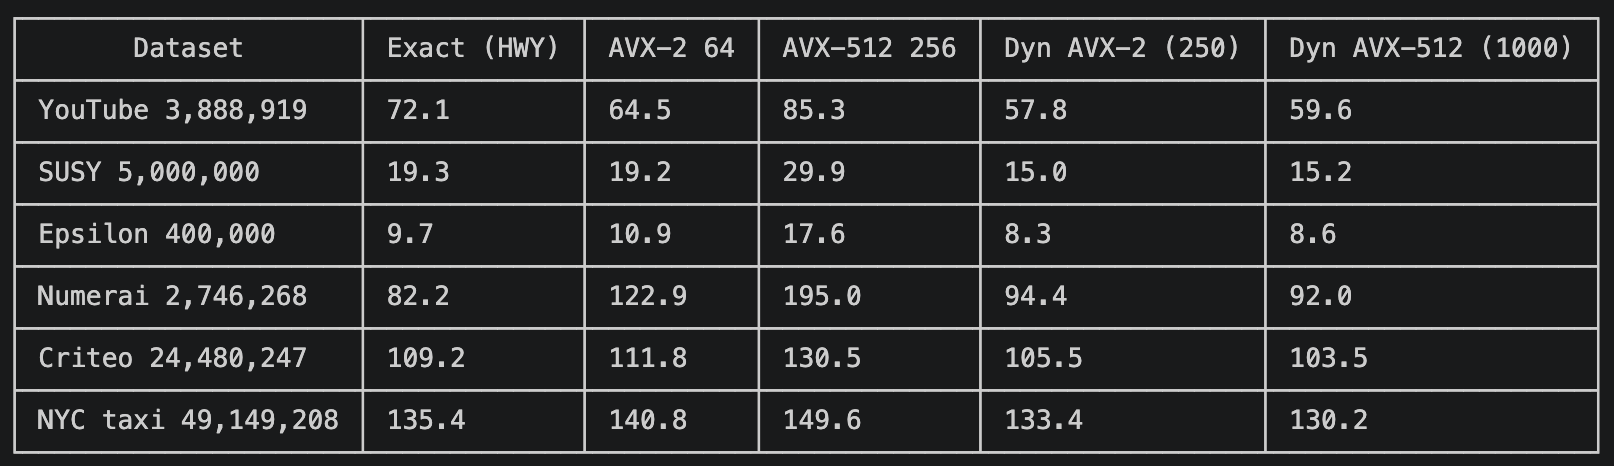
\includegraphics[width=\linewidth]{notes/figures/slow-natural-big.png}
    \caption{HWY is surprisingly fast on the largest datasets - \textit{AL: why?} Bcs. those datasets have ties (not continuous). HWY has a fast-path/short-circuit for ties. }
    \label{fig:hwy-on-discretized-numeric}
\end{figure}

\subsection{Ranking - LambdaMART}

Istella22~\cite{dato_istella22_2022} - 12m web documents, 220 hand-crafted features. Raw docs available

\subsection{Embedding - Extends Tabular to Multimodal}
\textit{Text + LLM embeddings is a strong GBT use case. Tabular structure gives benefit \cite{jiang2026multimodal}}


\subsubsection{Unimodal}

\begin{itemize}
    \item \textit{\href{https://research.google.com/youtube8m/download.html}{YouTube-8M} video-level 6m x 1152 - true embedding dataset, \textbf{but not Multimodal}}: 1152 embedding dims, no NaNs. ML task: \texttt{labels} (multi-class classification. I reduced to 1-vs-all). \textbf{Running now}
    \item \textbf{\textit{Richard MTEB}}. He uses proprietary, non-shareable Embedding + Tabular multimodals. MTEB is a benchmark of various tasks to test text embedding quality: classification, clustering, retrieval etc. e.g. \href{https://mteb-leaderboard.hf.space/tasks/Banking77Classification}{Bank phone call classification}. \textbf{\textit{We will need to create multimodal ourselves}}
\end{itemize}

\begin{figure}[htbp]
\centering
\begin{subfigure}[b]{0.405\linewidth}
    \centering
    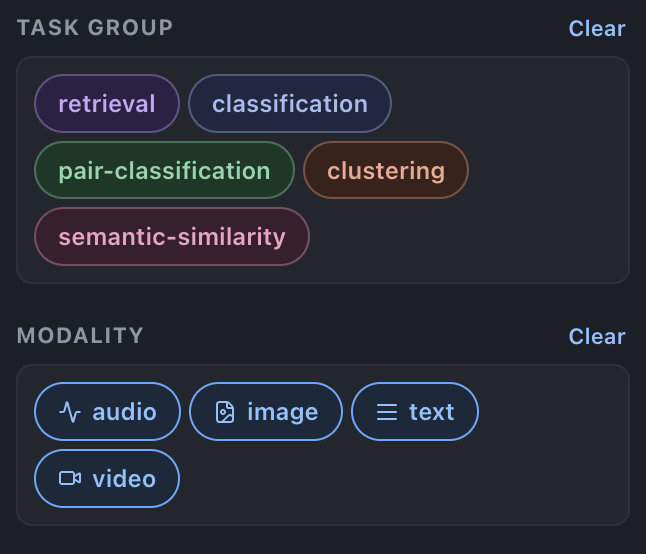
\includegraphics[width=\linewidth]{notes/figures/mteb-benchmark/modalities.png}
    \caption{\small MTEB task groups and modalities.}
    \label{fig:mteb-modalities}
\end{subfigure}
\hfill
\begin{subfigure}[b]{0.515\linewidth}
    \centering
    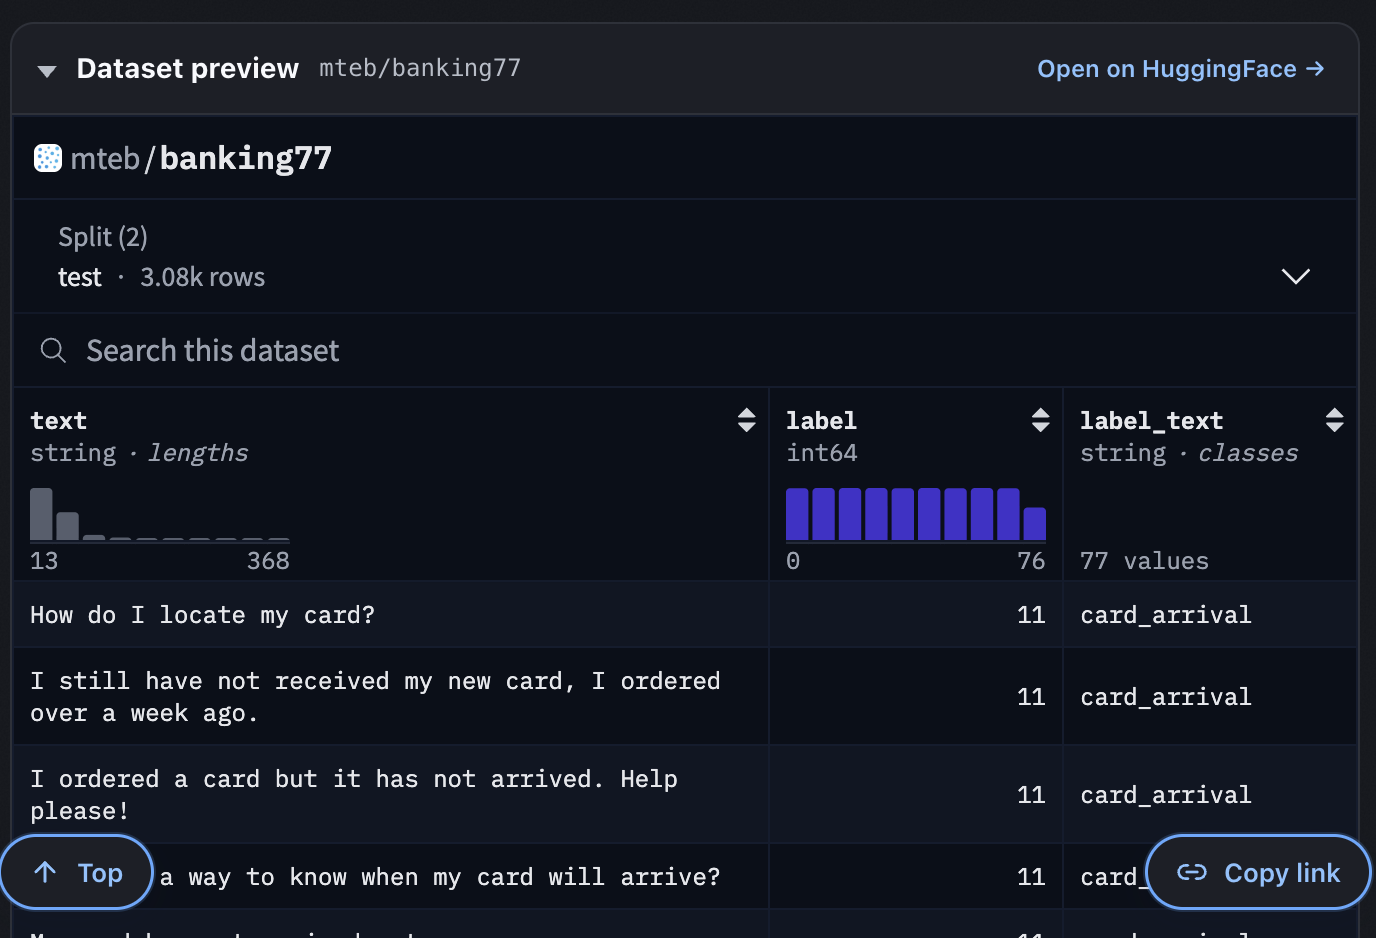
\includegraphics[width=\linewidth]{notes/figures/mteb-benchmark/mteb-example-banking77.png}
    \caption{\small\texttt{mteb/banking77}: 3.08k rows, 77 intent classes.}
    \label{fig:mteb-banking77}
\end{subfigure}

\vspace{1.5ex}

\begin{subfigure}[b]{0.48\linewidth}
    \centering
    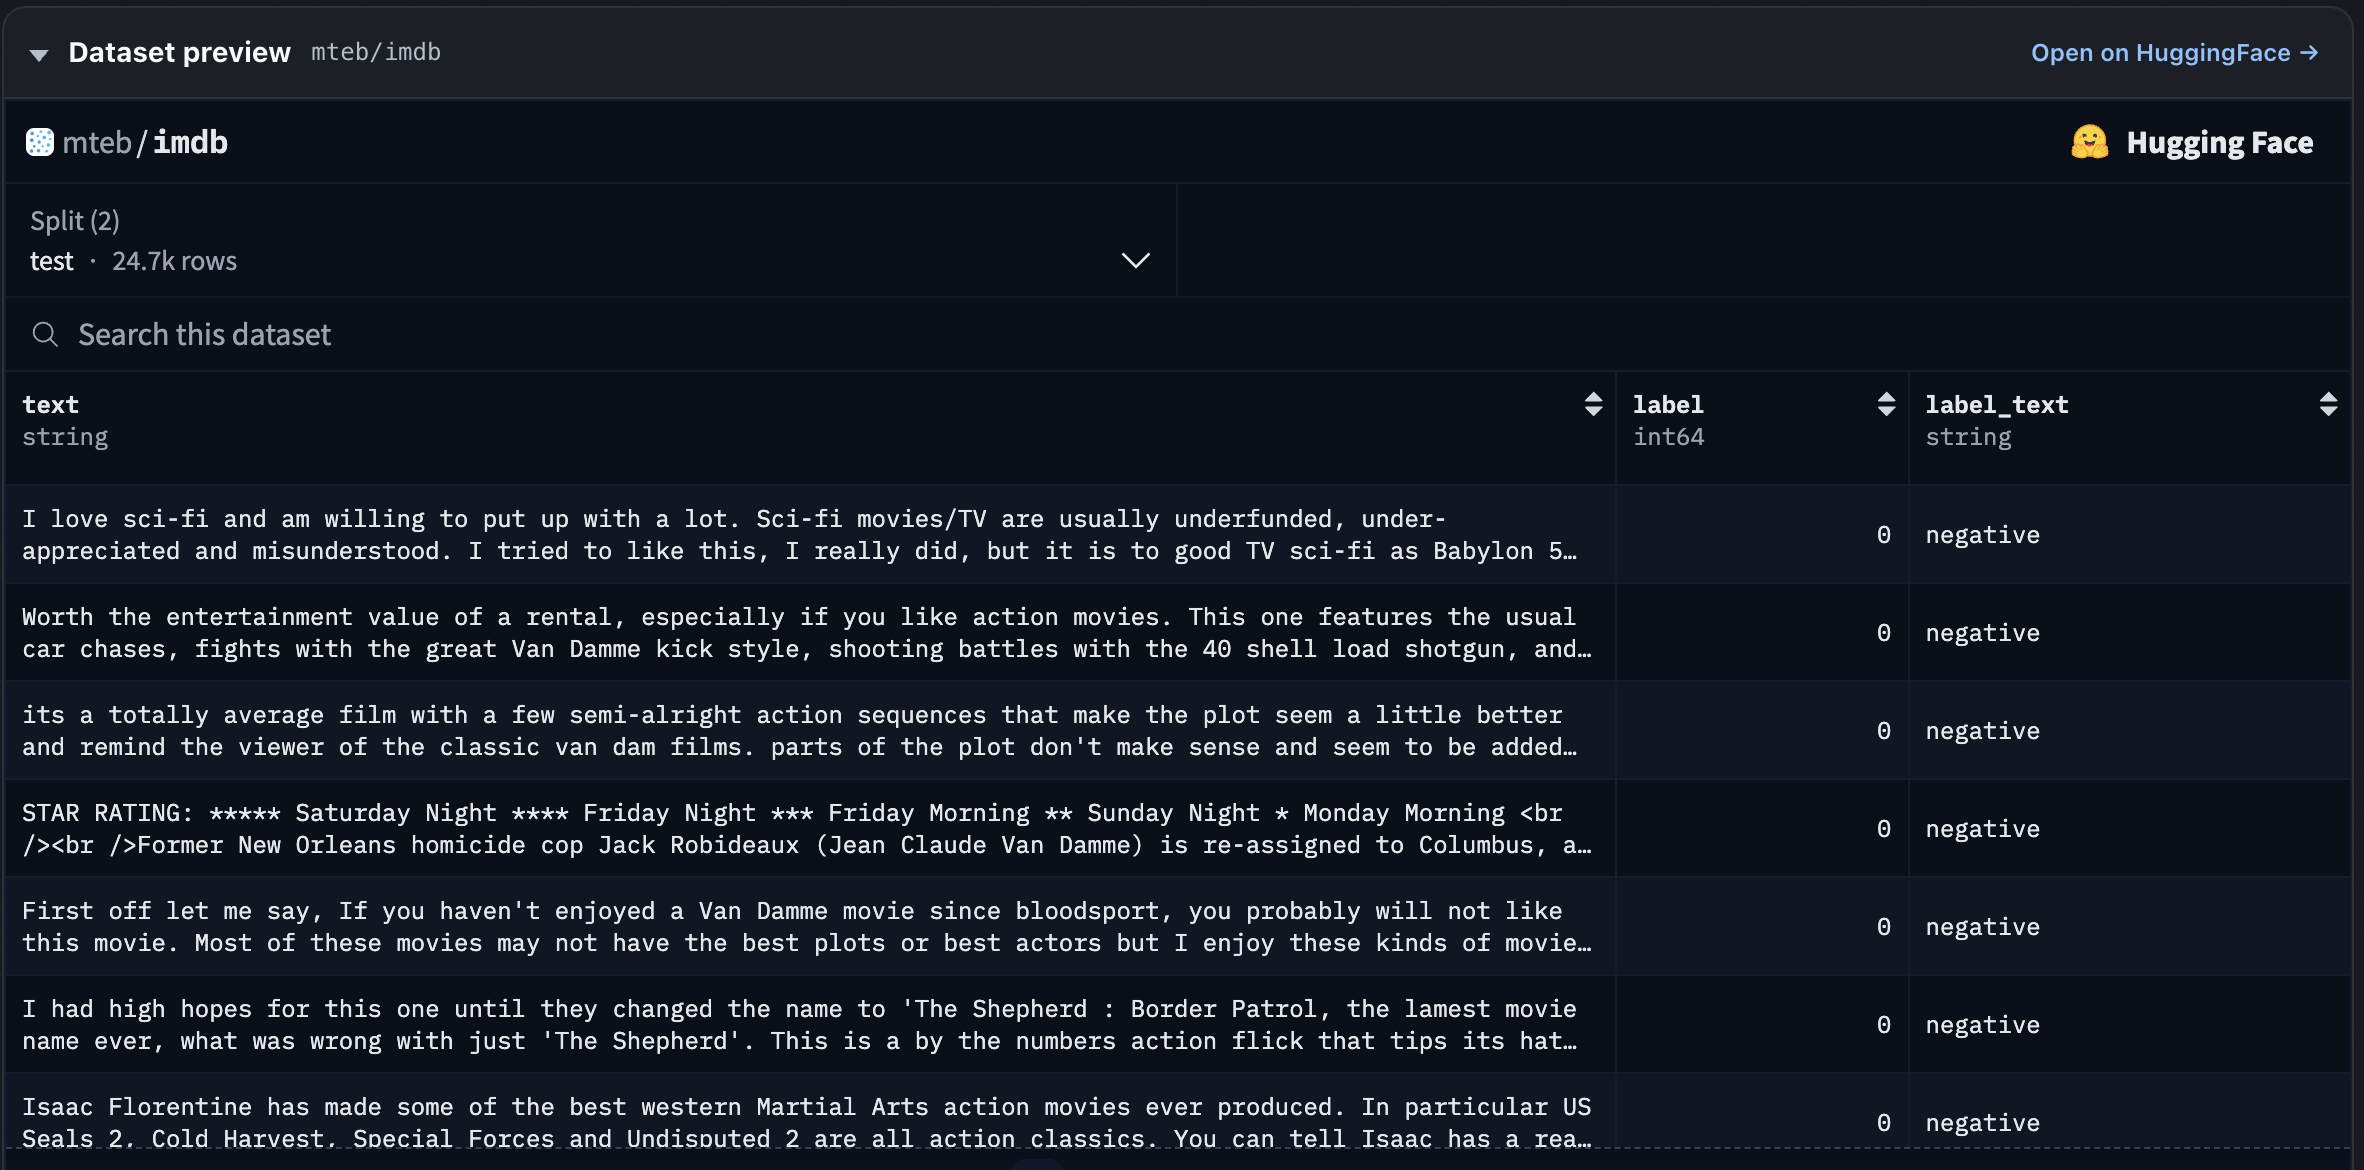
\includegraphics[width=\linewidth]{notes/figures/mteb-benchmark/imdb.png}
    \caption{\small\texttt{mteb/imdb}: 24.7k rows, binary sentiment.}
    \label{fig:mteb-imdb}
\end{subfigure}
\hfill
\begin{subfigure}[b]{0.48\linewidth}
    \centering
    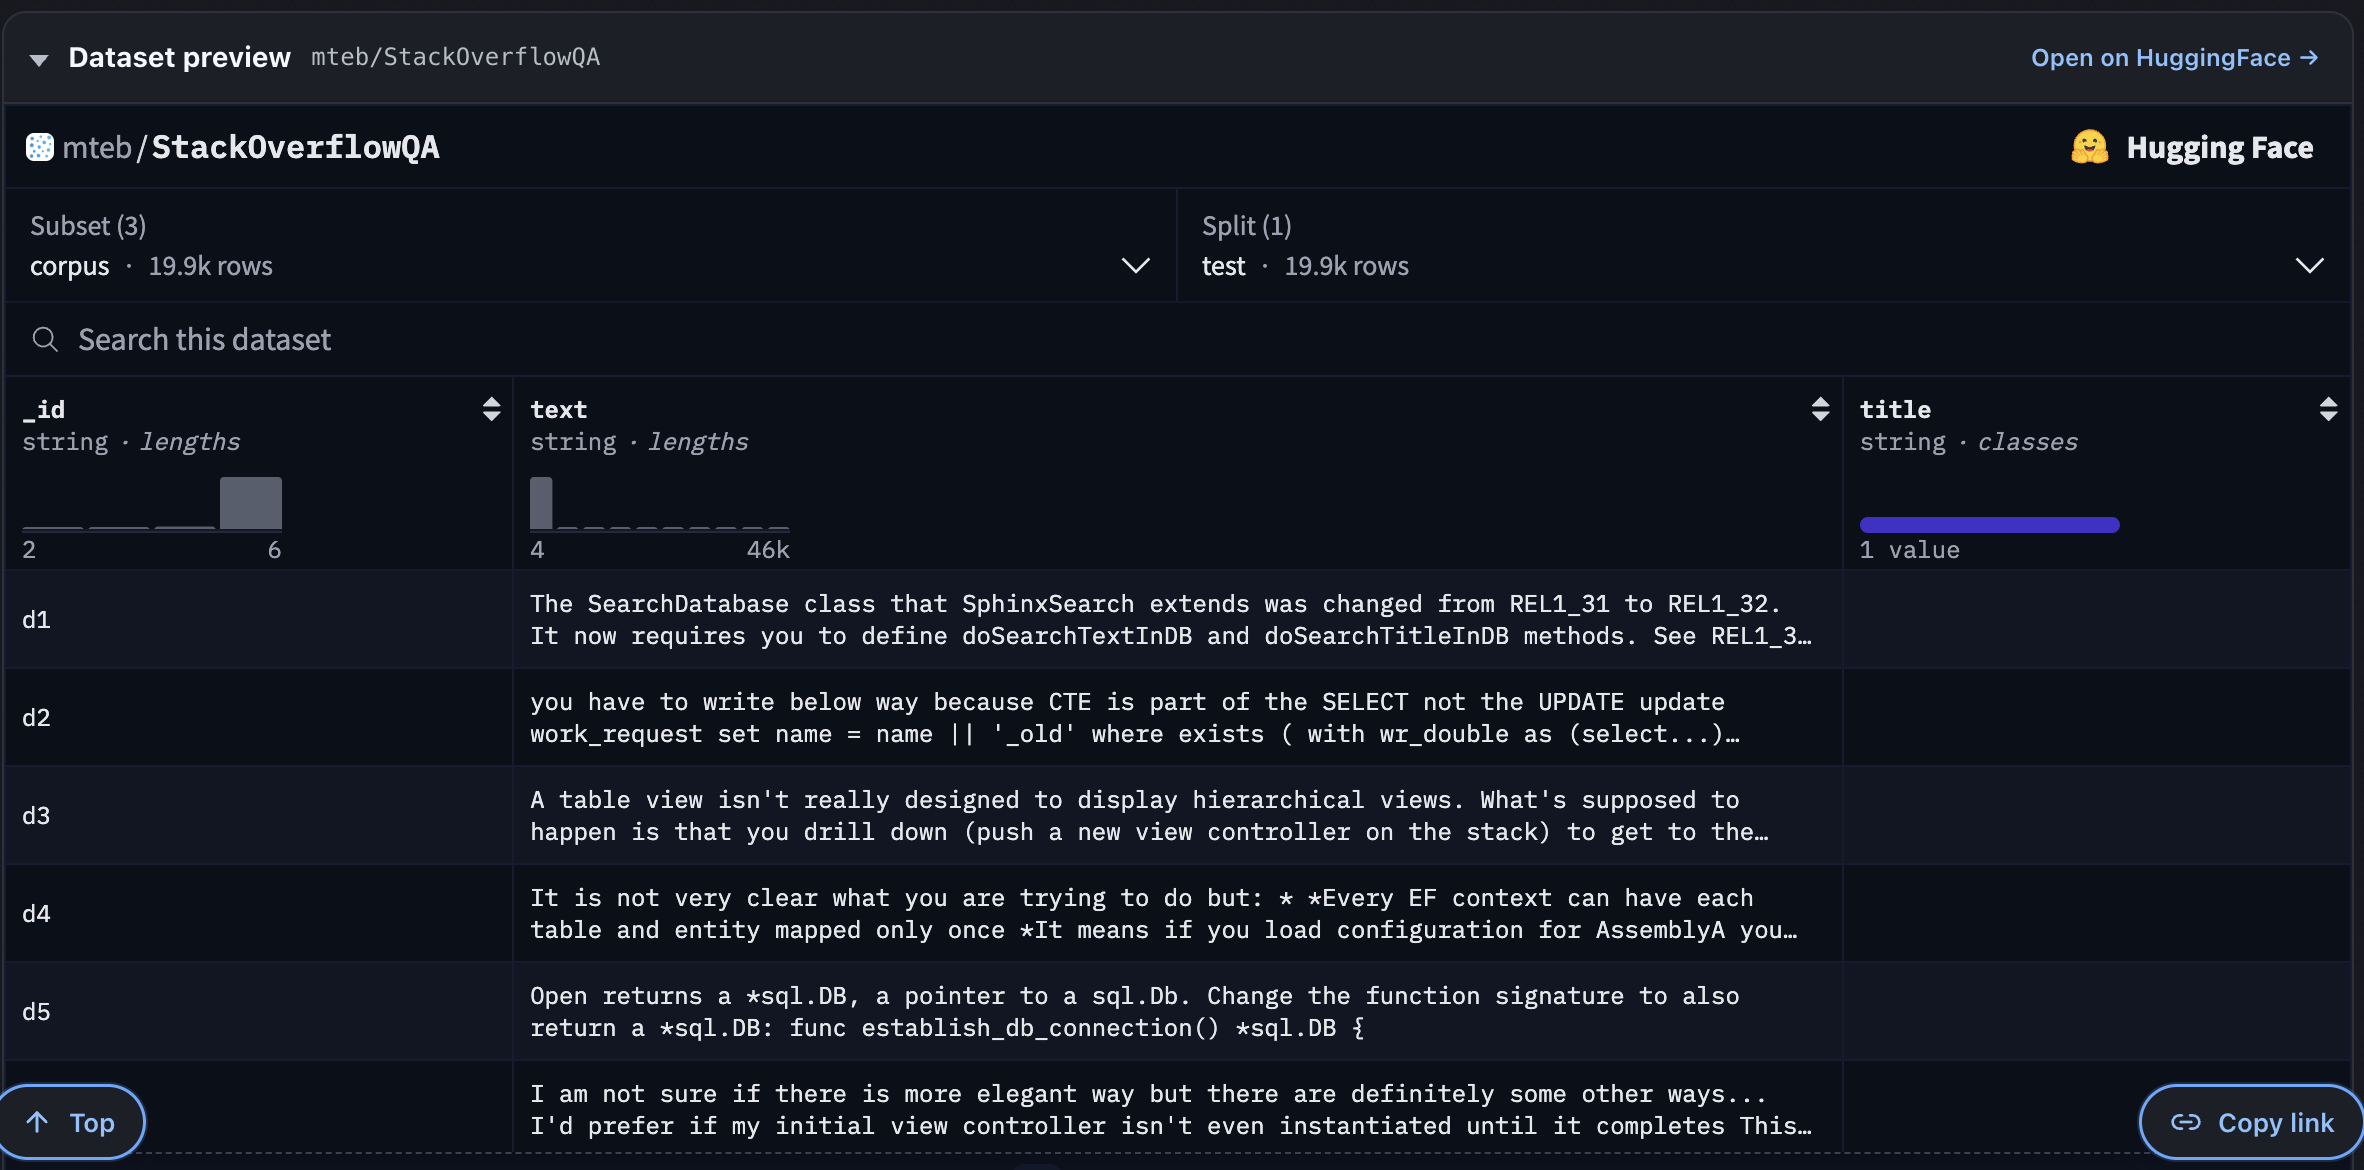
\includegraphics[width=\linewidth]{notes/figures/mteb-benchmark/stackoverflow.png}
    \caption{\small\texttt{mteb/StackOverflowQA}: 19.9k-row corpus.}
    \label{fig:mteb-stackoverflow}
\end{subfigure}
\caption{MTEB: task groups and modalities (a), and three dataset previews (b--d), each a text column plus label/metadata columns, embedded into numeric features.}
\label{fig:mteb-examples}
\end{figure}

\begin{figure}
    \centering
    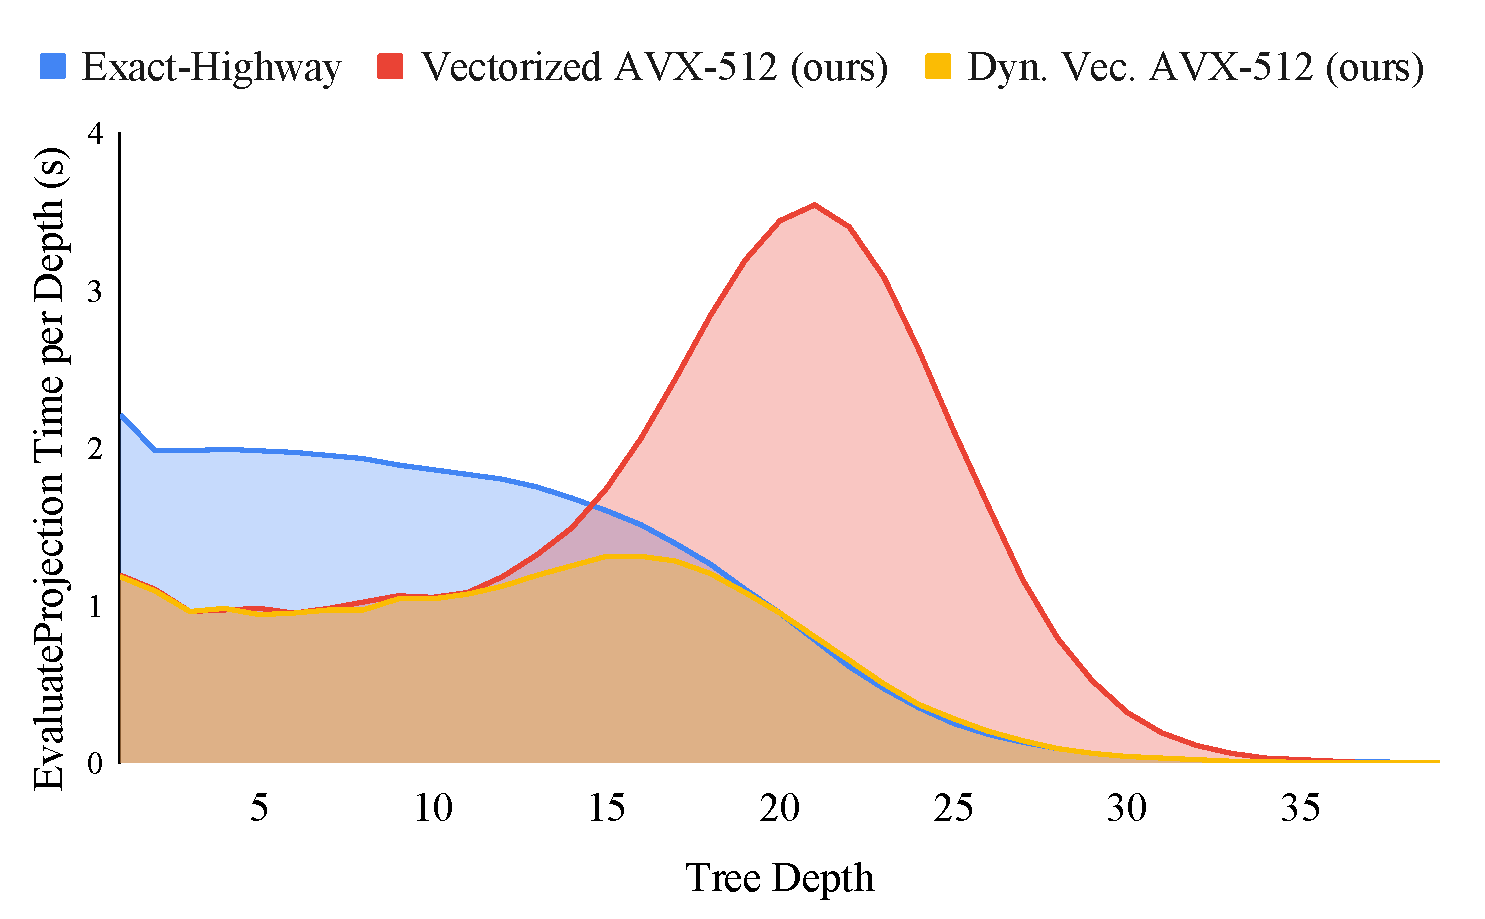
\includegraphics[width=0.75\linewidth]{figures/intro/dynamic/Youtube-8m-sporf.pdf}
    \caption{New Breakeven with Youtube-train (6m) looks exactly right}
\end{figure}

\subsubsection{Multimodal - needs handwork}

We need to manually create embeddings for these:

\begin{itemize}
    \item \href{https://www.kaggle.com/competitions/h-and-m-personalized-fashion-recommendations/data}{H\&M Personalized Fashion Recommendations} - good. Images, articles, customers, transactions. Can embed images.
    \item \href{https://www.aicrowd.com/challenges/amazon-kdd-cup-23-multilingual-recommendation-challenge}{Amazon KDD 2023 \& 2022 Cups} - Product details + text description (can be embedded)
    \item \href{https://www.kaggle.com/competitions/avito-demand-prediction/data}{Avito Demand Prediction} - same as Amazon 2022: Ads rec.
    \item Microsoft MIND News, Yelp Open data, etc. (didn't research)
    \item Good but small: [Google Scholar] MulTABench \cite{arazi_multabench_2026}: Multimodal Tabular Benchmark - great but small: max 114,000 rows x 245 features, AutoML Bag of Tricks~\cite{tang_bag_2024} (20k rows), AutoGluon–TimeSeries~\cite{shchur_autogluon-timeseries_2023} (100k).
    \item {\color{gray}\href{https://www.kaggle.com/competitions/otto-recommender-system}{OTTO} - discarded, event clicks of "aid" (int), "ts" (float), "type" (str). nonsense for humans }
\end{itemize}


\section{Issues with Discretized Datasets}

Criteo, NYC taxi, Numerai have lots of ties (ordinal categories set as numbers), and Highway is unusually fast due to some clever skipping of ties. See Fig.~\ref{fig:hwy-on-discretized-numeric}.


Went searching for more fully-numeric data:

\begin{itemize}
    \item ClimSim~\cite{yu2023climsim}[low-res], 744GB raw. Task: multi-output regression (weather prediction). Let's regress on only a single one of the Targets
    \item \href{https://www.kaggle.com/competitions/jane-street-real-time-market-data-forecasting/data}{Jane Street Kaggle 2024}
    \item \href{https://research.yandex.com/shifts/weather}{Yandex Weather Prediction} - 10m records, 111 features. Regression: Air Temp. at point
\end{itemize}



\appendix

Dataset treatment: agreeing to use Ordinal numbers for Categorical features, and NaNs are mean-imputed.

\bibliographystyle{plain}
\bibliography{main}

\end{document}
